% Artigo do TCC: Modelagem preditiva da produtividade da safra de soja no Rio Grande do Sul com aprendizado de máquina e dados agrometeorológicos
%
% Gerado a partir do template TemplateArtigoTCC_2026.tex (FCI/Mackenzie).
% Mesmo conteúdo da versão Word (artigo/Word/Artigo_TCC_Soja_RS.docx):
% ao mudar um texto ou um número, atualize as duas.
%
%% abtex2-modelo-artigo.tex, v-1.9.7 laurocesar
%% Copyright 2012-2018 by abnTeX2 group at http://www.abntex.net.br/ 
%%
%% This work may be distributed and/or modified under the
%% conditions of the LaTeX Project Public License, either version 1.3
%% of this license or (at your option) any later version.
%% The latest version of this license is in
%%   http://www.latex-project.org/lppl.txt
%% and version 1.3 or later is part of all distributions of LaTeX
%% version 2005/12/01 or later.
%%
%% This work has the LPPL maintenance status `maintained'.
%% 
%% The Current Maintainer of this work is the abnTeX2 team, led
%% by Lauro César Araujo. Further information are available on 
%% http://www.abntex.net.br/
%%
%% This work consists of the files abntex2-modelo-artigo.tex and
%% abntex2-modelo-references.bib
%%

% ------------------------------------------------------------------------
% ------------------------------------------------------------------------
% abnTeX2: Modelo de Artigo Acadêmico em conformidade com
% ABNT NBR 6022:2018: Informação e documentação - Artigo em publicação 
% periódica científica - Apresentação
% ------------------------------------------------------------------------
% ------------------------------------------------------------------------

% ------------------------------------------------------------------------
% ------------------------------------------------------------------------
% Este template foi alterado pelo Prof. Dr. Gustavo Scalabrini Sampaio
% da Faculdade de Computação e Informática (FCI) para atender os
% trabalhos de conclusão de curso da unidade acadêmica. 2025.
% ------------------------------------------------------------------------
% ------------------------------------------------------------------------

\documentclass[
	% -- opções da classe memoir --
	article,			% indica que é um artigo acadêmico
	11pt,				% tamanho da fonte
	oneside,			% para impressão apenas no recto. Oposto a twoside
	a4paper,			% tamanho do papel. 
	% -- opções da classe abntex2 --
	%chapter=TITLE,		% títulos de capítulos convertidos em letras maiúsculas
	%section=TITLE,		% títulos de seções convertidos em letras maiúsculas
	%subsection=TITLE,	% títulos de subseções convertidos em letras maiúsculas
	%subsubsection=TITLE % títulos de subsubseções convertidos em letras maiúsculas
	% -- opções do pacote babel --
	english,			% idioma adicional para hifenização
	brazil,				% o último idioma é o principal do documento
	sumario=tradicional
	]{abntex2}


% ---
% PACOTES
% ---

% ---
% Pacotes fundamentais 
% ---
\usepackage{lmodern}			% Usa a fonte Latin Modern
\usepackage[T1]{fontenc}		% Selecao de codigos de fonte.
\usepackage[utf8]{inputenc}		% Codificacao do documento (conversão automática dos acentos)
\usepackage{indentfirst}		% Indenta o primeiro parágrafo de cada seção.
\usepackage{nomencl} 			% Lista de simbolos
\usepackage{color}				% Controle das cores
\usepackage{graphicx}			% Inclusão de gráficos
\usepackage{microtype} 			% Para melhorias de justificação
\usepackage{hyperref}           % Habilita links e referências
% ---

% --- Header e Footer ---


\setlength{\headheight}{36pt}
\setlength{\headsep}{10pt}


\makepagestyle{meuestilo}
\makeevenhead{meuestilo}{
\includegraphics[height=1.1cm]{FCI.png}}{}{\thepage}
\makeoddhead {meuestilo}{
\includegraphics[height=1.1cm]{FCI.png}}{}{\thepage}


\makeheadrule{meuestilo}{\textwidth}{0.4pt}


\pagestyle{meuestilo}
% Para páginas "plain" (como início de capítulo/título):
\aliaspagestyle{chapter}{meuestilo}
\aliaspagestyle{plain}{meuestilo}


% Pacotes de citações
% ---
%\usepackage[brazilian,hyperpageref]{backref}	 % Paginas com as citações na bibl
\usepackage[alf]{abntex2cite}	% Citações padrão ABNT
% ---

% ---
% Configurações do pacote backref
% Usado sem a opção hyperpageref de backref
%\renewcommand{\backrefpagesname}{Citado na(s) página(s):~}
% Texto padrão antes do número das páginas
%\renewcommand{\backref}{}
% Define os textos da citação
%\renewcommand*{\backrefalt}[4]{
%	\ifcase #1 %
%		Nenhuma citação no texto.%
%	\or
%		Citado na página #2.%
%	\else
%		Citado #1 vezes nas páginas #2.%
%	\fi}%
% ---

% --- Informações de dados para CAPA e FOLHA DE ROSTO ---


\titulo{Modelagem preditiva da produtividade da safra de soja no Rio Grande do Sul com aprendizado de máquina e dados agrometeorológicos}
\def \theforeigntitle{Predictive modeling of soybean yield in Rio Grande do Sul with machine learning and agrometeorological data}

\autor{Nome Aluno Um \textsuperscript{1} 
\and Nome Aluno Dois \textsuperscript{1}
\and Nome Aluno Três \textsuperscript{1}
\and Nome Aluno Quatro \textsuperscript{1}
\and Nome Professor Orientador \textsuperscript{1,2} \\
\\ 
\textsuperscript{1}Faculdade de Computação e Informática (FCI) \\ Universidade Presbiteriana Mackenzie São Paulo, SP – Brasil \\ 
\\
\textsuperscript{2}Programa de pós-graduação em Computação Aplicada (quando houver) \\ Universidade Presbiteriana Mackenzie São Paulo, SP – Brasil 
\\
\\
\url{aluno.um, aluno.dois@mackenzista.com.br}
\\
\url{professor.orientador@mackenzie.br}}

\data{2026}
% ---

% ---
% Configurações de aparência do PDF final

% alterando o aspecto da cor azul
\definecolor{blue}{RGB}{41,5,195}

% informações do PDF
\makeatletter
\let\@fnsymbol\@arabic
\hypersetup{
     	%pagebackref=true,
		%pdftitle={\@title}, 
		%pdfauthor={\@author},
    	%pdfsubject={Modelo de artigo científico com abnTeX2},
	    %pdfcreator={LaTeX with abnTeX2},
		%pdfkeywords={abnt}{latex}{abntex}{abntex2}{atigo científico}, 
		colorlinks=true,       		% false: boxed links; true: colored links
    	linkcolor=blue,          	% color of internal links
    	citecolor=blue,        		% color of links to bibliography
    	%filecolor=magenta,         % color of file links
		urlcolor=blue,
		%bookmarksdepth=4
}
\makeatother
% --- 

% ---
% compila o indice
% ---
\makeindex
% ---

% ---
% Altera as margens padrões
% ---
\setlrmarginsandblock{3cm}{3cm}{*}
\setulmarginsandblock{3cm}{3cm}{*}
\checkandfixthelayout
% ---

% --- 
% Espaçamentos entre linhas e parágrafos 
% --- 

% O tamanho do parágrafo é dado por:
\setlength{\parindent}{1.3cm}

% Controle do espaçamento entre um parágrafo e outro:
\setlength{\parskip}{0.2cm}  % tente também \onelineskip

% Espaçamento simples
\SingleSpacing


% ----
% Início do documento
% ----
\begin{document}

\selectlanguage{brazil}
\frenchspacing

\maketitle

% resumo em português
\begin{resumoumacoluna}
\textit{A produtividade da soja no Rio Grande do Sul varia fortemente entre as safras, sobretudo pelas secas de verão associadas à La Niña, e o rendimento oficial por município só é divulgado pelo IBGE cerca de 17 meses após a colheita. Esta pesquisa, aplicada e quantitativa, desenvolve e avalia modelos de aprendizado de máquina supervisionado para prever, em 31 de março e apenas com dados já publicados nessa data, o rendimento da soja de cada município gaúcho. Foram integrados o rendimento municipal do IBGE (2000--2025), o clima diário do INMET e do NASA POWER, o índice ONI e um balanço hídrico do solo, e cada previsão soma ao patamar do município um desvio explicado pelo clima. Regressão linear, Random Forest e Gradient Boosting foram comparados com linhas de base históricas em validação temporal (teste 2021--2025) e deixando uma safra de fora. A hipótese de que os modelos ensemble superariam a regressão linear não se confirmou: o melhor modelo foi uma regressão linear com clima em grade e um termo de seca extrema, com RMSE de 772 e 626 kg/ha (R\textsuperscript{2} de 0,28 e 0,40), erro 11\% e 31\% menor que o da média histórica, enquanto o Gradient Boosting teve RMSE de 958 e 698 kg/ha. Para a safra 2026, o modelo previu 2.097 kg/ha, 23\% abaixo da estimativa do IBGE; para 2027, sob El Niño, a perspectiva é de 2.831 kg/ha. Com poucas safras, a representação do clima pesou mais que a escolha do algoritmo.}

 \vspace{\onelineskip}

 \noindent
 \textbf{Palavras-chave}: soja; previsão de produtividade; aprendizado de máquina; balanço hídrico; dados agrometeorológicos.
\end{resumoumacoluna}

% resumo em inglês
\renewcommand{\resumoname}{Abstract}
\begin{resumoumacoluna}
 \begin{otherlanguage*}{english}
\textit{Soybean yield in Rio Grande do Sul, Brazil, varies widely between seasons, mainly due to summer droughts associated with La Niña, and official municipal yields are released by IBGE about 17 months after harvest. This applied, quantitative study develops and evaluates supervised machine learning models that forecast, on March 31 and using only data already published by then, the soybean yield of each municipality in the state. Municipal yields from IBGE (2000--2025), daily weather from INMET and NASA POWER, the ONI index and a soil water balance were integrated, and each forecast was structured as the sum of a municipal baseline and a deviation explained by the weather of each crop stage. Linear regression, Random Forest and Gradient Boosting were compared with historical baselines in a temporal validation (2021--2025 test) and in leave-one-season-out validation. The hypothesis that ensemble models would outperform linear regression was not confirmed: the best model was a linear regression with gridded weather and an extreme-drought term, with RMSE of 772 and 626 kg/ha (R\textsuperscript{2} of 0.28 and 0.40), 11\% and 31\% lower than the historical mean, while Gradient Boosting reached RMSE of 958 and 698 kg/ha. For the 2026 season, the model forecast 2,097 kg/ha, 23\% below the IBGE estimate; for 2027, under El Niño, the outlook is 2,831 kg/ha. With few seasons, the representation of weather mattered more than the choice of algorithm.}

   \vspace{\onelineskip}

   \noindent
   \textbf{Keywords}: soybean; crop yield forecasting; machine learning; soil water balance; agrometeorological data.
 \end{otherlanguage*}
\end{resumoumacoluna}

% ----------------------------------------------------------
% ELEMENTOS TEXTUAIS
% ----------------------------------------------------------
\textual

\section{Introdução}\label{sec:intro}

A soja é uma das principais culturas do agronegócio brasileiro, e o Rio Grande do Sul (RS) está entre os maiores produtores do país. No estado, o rendimento varia muito de uma safra para outra, sobretudo por secas de verão: o rendimento médio estadual foi de 3.343 kg/ha em 2021 e de 1.508 kg/ha em 2022, e a média dos municípios chegou a 662 kg/ha na seca de 2005. Essa variação depende da chuva, da temperatura, de veranicos e de fenômenos de grande escala como El Niño e La Niña \cite{pilau2022,noia2020}, e ganha importância com o aumento da variabilidade climática.

O resultado oficial por município, a Produção Agrícola Municipal (PAM) do Instituto Brasileiro de Geografia e Estatística (IBGE), só é divulgado em setembro do ano seguinte à colheita \cite{ibgepam2024}. Até lá, cooperativas, produtores, seguradoras e órgãos públicos planejam crédito, logística e comercialização sem uma estimativa municipal do rendimento. O problema de pesquisa é, portanto: é possível estimar o rendimento da soja de cada município gaúcho antes do fim da colheita, apenas com dados públicos disponíveis na data da previsão, com erro menor que o de referências históricas simples?

Revisões da literatura indicam que modelos de aprendizado de máquina baseados em árvores de decisão, como Random Forest e Gradient Boosting, estão entre os mais usados e costumam superar a regressão linear na previsão de safras \cite{vanklompenburg2020,jeong2016,vonbloh2023}. Esses resultados vêm, em geral, de bases maiores e de validações que nem sempre respeitam a data em que cada dado se torna público. Há menos evidência sobre o desempenho desses modelos num cenário de dados limitados — cerca de 20 safras e 5 a 8 mil pares município--safra — e com a restrição de usar só o que já foi publicado no momento da previsão. A hipótese inicial deste trabalho foi que os modelos de vertente \emph{ensemble} (Random Forest e Gradient Boosting) superariam a regressão linear em RMSE e R\textsuperscript{2}.

O objetivo geral é desenvolver e avaliar modelos de aprendizado de máquina supervisionado que prevejam, em 31 de março, o rendimento da soja (kg/ha) de cada município do RS a partir de dados agrometeorológicos públicos. Os objetivos específicos são:

\begin{itemize}
\item integrar, por município e safra, o rendimento do IBGE (2000--2025), o clima diário do INMET e do NASA POWER e o índice ONI;
\item construir variáveis climáticas por subperíodo do ciclo da soja e um balanço hídrico do solo;
\item comparar regressão linear, Random Forest e Gradient Boosting com linhas de base históricas, em validação temporal e deixando uma safra de fora;
\item identificar os fatores climáticos mais associados à variação do rendimento;
\item prever a safra 2026, compará-la com a estimativa oficial do IBGE e montar a perspectiva da safra 2027 por cenários climáticos.
\end{itemize}

Uma estimativa antecipada e municipal do rendimento pode sinalizar os municípios sob risco de quebra e apoiar decisões de planejamento agrícola, em linha com o Objetivo de Desenvolvimento Sustentável 2 (fome zero e agricultura sustentável). O objetivo é um indicador regional, transparente e reprodutível, construído só com dados públicos, e não a previsão de uma propriedade específica. O trabalho contribui com uma base municipal integrada e versionada, com uma comparação de algoritmos sob uma validação que respeita a data de publicação dos dados e com uma previsão real, fora da amostra, da safra 2026, comparada à estimativa oficial.

O artigo está organizado da seguinte forma: a Seção \ref{sec:referencial} apresenta o referencial teórico; a Seção \ref{sec:metodologia} descreve os dados, a construção das variáveis, os modelos e a validação; a Seção \ref{sec:resultados} apresenta e discute os resultados, incluindo a previsão da safra 2026 e a perspectiva da safra 2027; e a Seção \ref{sec:conclusao} traz as conclusões e os trabalhos futuros.

\section{Referencial Teórico}\label{sec:referencial}

\subsection{Clima e produtividade da soja no Rio Grande do Sul}

No RS, a soja é semeada de outubro a dezembro, floresce e enche os grãos de dezembro a fevereiro e é colhida de março a maio. A falta de água no período de floração e enchimento de grãos é a principal causa de perda de rendimento, pois reduz o número e o peso dos grãos. A chuva da primavera e do verão no Sul do Brasil é modulada pelo El Niño--Oscilação Sul (ENOS): a La Niña tende a trazer chuva abaixo da média, e o El Niño, acima. \citeonline{pilau2022} associam a variabilidade da chuva ligada ao ENOS a perdas de rendimento da soja no estado, e \citeonline{noia2020} mostram que a fase do ENOS e a data de semeadura alteram o rendimento e a ocorrência de eventos extremos no Sul do Brasil. A fase do ENOS é medida pelo Oceanic Niño Index (ONI), a anomalia trimestral da temperatura do Pacífico equatorial \cite{noaa}.

A chuva, porém, não mede diretamente a água disponível para a planta. O balanço hídrico do solo compara a água que entra (chuva) com a que sai por evapotranspiração. O método de referência para a evapotranspiração é o de Penman--Monteith padronizado pela FAO \cite{allen1998}, que exige radiação, vento e umidade; quando só a temperatura está disponível de forma confiável, o método de \citeonline{hargreaves1985} é uma alternativa usual. Representando o solo como um reservatório de capacidade de água disponível (CAD) finita, a demanda não atendida quando ele se esgota é o déficit hídrico, uma medida mais próxima do estresse da cultura do que o total de chuva.

\subsection{Aprendizado de máquina na previsão de safras}

No aprendizado supervisionado, um modelo aprende uma função que relaciona entradas a uma saída conhecida a partir de exemplos rotulados; quando a saída é contínua, como o rendimento em kg/ha, o problema é de regressão \cite{russell2021}. Na revisão sistemática de \citeonline{vanklompenburg2020}, redes neurais, regressão linear, Random Forest e Gradient Boosting aparecem entre os algoritmos mais usados para prever produtividade, e temperatura, chuva e tipo de solo, entre as variáveis mais frequentes. \citeonline{jeong2016} compararam Random Forest e regressão linear múltipla na previsão de produtividade de várias culturas, em escala global e regional, e obtiveram erros menores com o Random Forest; \citeonline{vonbloh2023} aplicaram aprendizado de máquina à previsão da produtividade da soja no Brasil. Esses trabalhos motivaram a hipótese deste estudo.

A \textbf{regressão linear} estima o rendimento como uma soma ponderada das variáveis. É interpretável — cada coeficiente indica a variação associada a uma unidade da variável — e pode representar relações não lineares por termos transformados, como um quadrado ou um termo de limiar max(0, x $-$ c), que vale zero abaixo de c e cresce linearmente acima dele. O \textbf{Random Forest} \cite{breiman2001} combina centenas de árvores de decisão treinadas em amostras \emph{bootstrap} e com subconjuntos aleatórios de variáveis (\emph{bagging}), o que reduz a variância. O \textbf{Gradient Boosting} \cite{friedman2001} constrói as árvores em sequência, cada uma ajustada ao erro das anteriores, controlado por uma taxa de aprendizado. Os dois capturam interações sem especificação prévia, mas, como a previsão de uma árvore é uma média de valores vistos no treino, não extrapolam para condições mais extremas que as do histórico. Os três algoritmos estão implementados na biblioteca scikit-learn \cite{pedregosa2011}.

\subsection{Validação e interpretação de modelos}

Em dados temporais, a divisão aleatória entre treino e teste deixa o modelo ver safras posteriores às que prevê e superestima o desempenho. São preferíveis a validação temporal, que treina com o passado e testa no futuro, e a validação que deixa um grupo de fora, em que cada safra inteira é prevista por um modelo treinado com as demais. Para interpretar as previsões, os valores SHAP \cite{lundberg2017} decompõem cada previsão em contribuições aditivas das variáveis; num modelo linear, a contribuição de uma variável é o coeficiente multiplicado pela diferença entre o seu valor e a média do treino.

\section{Metodologia}\label{sec:metodologia}

\subsection{Tipo de pesquisa}

A pesquisa é aplicada e quantitativa, de caráter experimental computacional: modelos de regressão são treinados e comparados com dados históricos sob protocolos de validação definidos antes da análise. A modelagem foi conduzida em seis etapas, cada uma motivada pelo diagnóstico dos erros da anterior. A pesquisa não envolve seres humanos nem animais e usa apenas dados públicos agregados por município, sem dados pessoais, em conformidade com a Lei Geral de Proteção de Dados (LGPD).

\subsection{Dados e coleta}

Todas as fontes são públicas e oficiais (Tabela \ref{tab:fontes}). Os dados foram obtidos nos portais e serviços das instituições; o clima do NASA POWER, pela interface de programação do serviço, com o \emph{script} \path{dataset/baixar_nasa_power.py} do repositório. Área plantada, área colhida e produção da própria safra não são usadas como preditores, pois só são conhecidas depois da colheita.

\begin{table}[htbp]
\centering
\caption{Fontes de dados}
\label{tab:fontes}
\small
\begin{tabular}{|>{\raggedright\arraybackslash}p{3.19cm}|>{\raggedright\arraybackslash}p{6.01cm}|>{\raggedright\arraybackslash}p{4.13cm}|}
\hline
\textbf{Fonte} & \textbf{Conteúdo} & \textbf{Uso} \\ \hline
IBGE/SIDRA -- PAM, Tabela 1612 \cite{ibge} & Rendimento (kg/ha), área e produção de soja por município do RS, 2000--2025 & Variável-alvo e patamar do município \\ \hline
IBGE/SIDRA -- LSPA, Tabela 6588 \cite{ibgelspa} & Estimativa mensal do rendimento da safra corrente no RS & Referência para a safra 2026 \\ \hline
NOAA/CPC -- ONI \cite{noaa} & Índice trimestral do ENOS (El Niño/La Niña) & Fase do ENOS por safra; cenários de 2027 \\ \hline
INMET/BDMEP \cite{inmet} & Chuva, temperaturas e umidade diárias de 45 estações automáticas do RS & Clima das Etapas 1 a 4 \\ \hline
NASA POWER \cite{nasapower} & Chuva, temperaturas e ponto de orvalho diários em grade (0,5\textdegree{} $\times$ 0,625\textdegree{}; 87 células), 2000 a maio/2026, sem falhas & Clima das Etapas 5 e 6 e das previsões \\ \hline
IBGE -- Localidades \cite{ibgelocalidades} & Mesorregião de cada município & Erro e previsão por região \\ \hline
\end{tabular}
\fonte{Elaborado pelos autores (2026).}
\end{table}

\subsection{Pré-processamento e integração}

As bases foram integradas em Python num painel de 12.922 pares município--safra (497 municípios, 2000--2025). Pelos símbolos do SIDRA, 10.540 pares têm rendimento, 2.308 são de municípios que não plantaram soja naquele ano, 54 não têm dado disponível e 20 são perdas totais (área plantada sem área colhida, 10 delas em 2005), que ficam fora do modelo porque o rendimento não é definido. A safra Y é a colhida no ano Y (a safra 2026 corresponde ao ciclo 2025/26).

O clima diário foi associado a cada município de duas formas: pela estação do INMET mais próxima, com exigência de cobertura mínima de dados no período, e pela célula do NASA POWER que contém a sede do município. A base de modelagem exige ainda o patamar do município, disponível a partir da safra 2006. Com o INMET, ela tem 5.236 pares (448 municípios); com o NASA POWER, 8.261 pares (449 municípios), todas as linhas com rendimento desde 2006.

\subsection{Restrição temporal da previsão}

A previsão da safra Y é emitida em 31 de março de Y, cerca de um mês antes do fim da colheita, e só usa informações disponíveis nessa data: o clima de outubro a março e o ONI. Como a PAM é divulgada em setembro do ano seguinte à colheita — a PAM 2024 saiu em 11 de setembro de 2025 \cite{ibgepam2024} —, em março de Y a última safra publicada é Y$-$2 (Tabela \ref{tab:disponiveis}). Usar a safra Y$-$1 daria ao modelo um dado que só existirá seis meses depois da previsão. Na validação histórica vale a mesma regra: a safra 2022, por exemplo, é prevista com as safras publicadas até 2020.

\begin{table}[htbp]
\centering
\caption{Dados de rendimento disponíveis na data de cada previsão}
\label{tab:disponiveis}
\small
\begin{tabular}{|>{\centering\arraybackslash}p{2.70cm}|>{\centering\arraybackslash}p{3.28cm}|>{\centering\arraybackslash}p{3.66cm}|>{\centering\arraybackslash}p{3.28cm}|}
\hline
\textbf{Safra prevista} & \textbf{Emissão da previsão} & \textbf{Última PAM publicada} & \textbf{Patamar (5 safras)} \\ \hline
2026 & 31/03/2026 & 2024 (set/2025) & 2020--2024 \\ \hline
2027 & 31/03/2027 & 2025 (set/2026) & 2021--2025 \\ \hline
\end{tabular}
\fonte{Elaborado pelos autores (2026).}
\end{table}

\subsection{Estrutura da previsão: patamar e desvio climático}

Cada previsão é a soma de um \textbf{patamar} — o rendimento esperado do município numa safra normal — e de um \textbf{desvio} explicado pelo clima da safra:

\begin{equation}
\hat{y}_{m,Y} = P_{m,Y} + f(\mathbf{x}_{m,Y}), \qquad P_{m,Y} = \frac{1}{5}\sum_{k=2}^{6} y_{m,Y-k}
\end{equation}

em que m é o município, P é a média das cinco últimas safras publicadas e f é o modelo do desvio, aplicado às variáveis climáticas x. Quatro formas de patamar foram comparadas, todas com as safras publicadas: reta de tendência estadual, média móvel das cinco últimas safras do município, média olímpica dessas cinco safras e reta das dez últimas safras; a média móvel teve o melhor desempenho e foi adotada. O problema foi tratado como regressão em painel, e não como série temporal por município, porque cada município tem cerca de 26 safras, pouco para ajustar um ARIMA ou uma rede recorrente de forma confiável.

\subsection{Variáveis climáticas e balanço hídrico}

O clima diário foi agregado em três subperíodos do ciclo: outubro--novembro (semeadura), dezembro--fevereiro (floração e enchimento de grãos, o período crítico) e março (maturação). Para dezembro--fevereiro foram calculados também a maior sequência de dias secos, os dias com temperatura máxima $\geq$ 32\,\textdegree C e a umidade relativa mínima média; no NASA POWER, a umidade mínima foi estimada pelo ponto de orvalho e pela temperatura máxima \cite{allen1998}. A evapotranspiração de referência foi estimada pelo método de Hargreaves--Samani \cite{hargreaves1985}:

\begin{equation}
ET_o = 0{,}0023 \cdot 0{,}408\,R_a \cdot (T_{\mathrm{med}} + 17{,}8)\sqrt{T_{\mathrm{max}} - T_{\mathrm{min}}}
\end{equation}

em que R\emph{a} é a radiação no topo da atmosfera, calculada pela latitude e pelo dia do ano, e T são as temperaturas média, máxima e mínima do dia (\textdegree{}C). O solo foi representado como um reservatório com CAD de 75 mm, cheio em 1º de outubro; a demanda não atendida quando o reservatório se esgota é o déficit hídrico do dia, acumulado de dezembro a fevereiro. A sensibilidade à CAD (50 e 100 mm) não alterou os resultados.

\subsection{Modelos comparados}

A Tabela \ref{tab:modelos} lista os modelos. Nos termos de seca extrema, U é a umidade mínima e D o déficit hídrico de dezembro a fevereiro; U\textsubscript{20} e D\textsubscript{80} são os níveis que delimitam as 20\% safras mais secas do treino. Esses termos valem zero em safras normais e permitem que a perda cresça mais rápido na seca forte. Médias, limiares e penalizações são calculados apenas com o treino de cada rodada, e os hiperparâmetros das árvores foram fixados \emph{a priori} (Gradient Boosting: taxa de aprendizado 0,05 e até 500 iterações com parada antecipada; Random Forest: 500 árvores), para que as safras de teste não influenciem a escolha.

\begin{table}[htbp]
\centering
\caption{Modelos e linhas de base}
\label{tab:modelos}
\small
\begin{tabular}{|>{\raggedright\arraybackslash}p{3.19cm}|>{\raggedright\arraybackslash}p{2.82cm}|>{\raggedright\arraybackslash}p{7.33cm}|}
\hline
\textbf{Modelo} & \textbf{Tipo} & \textbf{Variáveis do desvio} \\ \hline
Média histórica & Linha de base & Média de todas as safras publicadas do município, sem clima \\ \hline
Última safra publicada & Linha de base & Rendimento da safra Y$-$2, sem clima \\ \hline
F & Regressão linear & Chuva de out--nov, chuva de dez--fev e seu quadrado, chuva de março, dias de calor e umidade mínima de dez--fev \\ \hline
H1 & Regressão linear & F + déficit hídrico de dez--fev \\ \hline
H2 & Regressão linear & H1 + max(0, U\textsubscript{20} $-$ U) + max(0, D $-$ D\textsubscript{80}) \\ \hline
\textbf{FL (final)} & \textbf{Regressão linear} & \textbf{F + max(0, D $-$ D\textsubscript{80})} \\ \hline
Random Forest & Árvores (\emph{bagging}) & Clima, ONI e efeito do município (Etapas 1 e 2) \\ \hline
GB -- Gradient Boosting & Árvores (\emph{boosting}) & Todas as variáveis climáticas, o ONI e o balanço hídrico \\ \hline
\end{tabular}
\nota{Na Etapa 5 também foram testadas a média de F e H2, uma regressão Ridge com as variáveis de H2 e F acrescida só do limiar de umidade.}
\fonte{Elaborado pelos autores (2026).}
\end{table}

\subsection{Validação e métricas}

Os dados nunca são divididos de forma aleatória. Foram usadas duas validações: (i) \textbf{corte temporal}, com treino até 2020 e teste em 2021--2025, que simula a previsão real nas safras mais recentes; e (ii) \textbf{deixando uma safra de fora}, em que cada safra de 2008 a 2025 é prevista por um modelo treinado com todas as demais, o que mede a estabilidade da relação entre clima e rendimento. Nas duas, o patamar usa só safras publicadas. As métricas, calculadas sobre os n pares município--safra avaliados, são:

\begin{equation}
\mathrm{RMSE} = \sqrt{\frac{1}{n}\sum_{i=1}^{n}(\hat{y}_i - y_i)^2}, \quad \mathrm{MAE} = \frac{1}{n}\sum_{i=1}^{n}|\hat{y}_i - y_i|, \quad R^2 = 1 - \frac{\sum_i(\hat{y}_i - y_i)^2}{\sum_i(y_i - \bar{y})^2}
\end{equation}

e o viés médio, $\Sigma$($\hat{y}$ $-$ y)/n. O R\textsuperscript{2} negativo indica erro maior que o de prever a média observada do próprio período avaliado. O modelo final é o de menor RMSE médio nas duas validações. Para facilitar a leitura, o desempenho também é expresso como acurácia, definida como 100\% menos o MAE relativo ao rendimento médio. O intervalo de 80\% das previsões vem dos percentis 10 e 90 do erro na validação deixando uma safra de fora, e a média estadual é ponderada pela área plantada, como na PAM.

\subsection{Ferramentas e reprodutibilidade}

A solução foi implementada em Python 3.13, com pandas e NumPy no tratamento dos dados, scikit-learn \cite{pedregosa2011} nos modelos, SciPy nos testes dos coeficientes e Matplotlib nos gráficos. Os notebooks de cada etapa (\path{analise_exploratoria} e \path{modelagem} a \path{modelagem_etapa6_previsao_2026_2027}), os dados brutos e processados e as versões das bibliotecas estão no repositório do projeto (\url{https://github.com/isah5/Projeto_Safra_de_Soja}), o que permite reproduzir todos os números deste artigo.

\section{Resultados e discussão}\label{sec:resultados}

\subsection{Análise exploratória}

O rendimento médio foi menor sob La Niña ($\approx$2.230 kg/ha) do que em safras neutras ($\approx$2.351 kg/ha) e sob El Niño ($\approx$2.462 kg/ha) (Figura \ref{fig:enos}), o que justifica o uso do ONI e a separação dos cenários de 2027 pela fase do ENOS. No nível município--safra, porém, a correlação do rendimento com o ONI é fraca ($\approx$0,16) e com a chuva total da safra é moderada ($\approx$0,38): variáveis agregadas simples não bastam, o que orientou as etapas seguintes.

\begin{figure}[htbp]
\centering
\caption{Rendimento médio da soja por fase do ENOS, classificada pelo ONI médio da safra (RS, 2000--2025)}
\label{fig:enos}
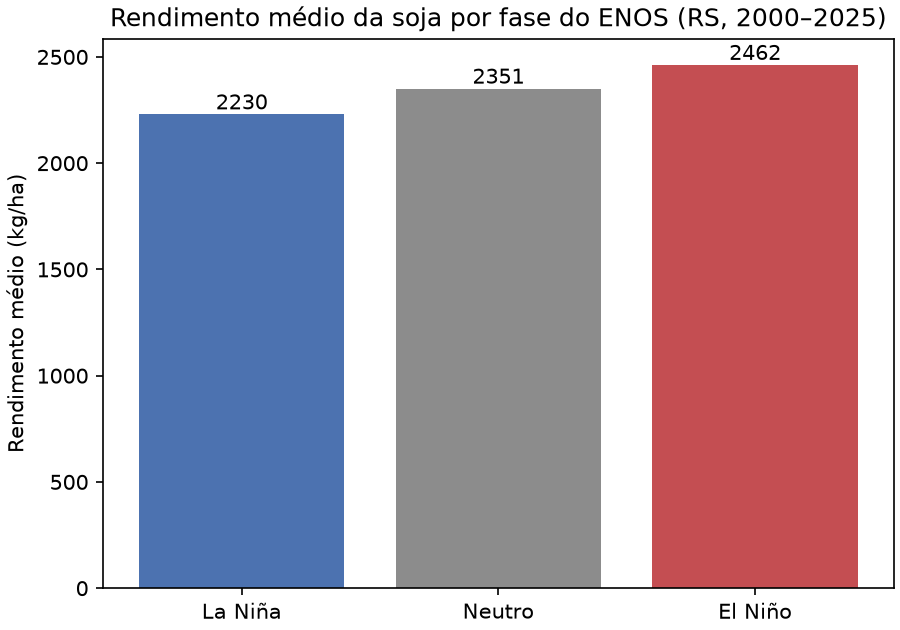
\includegraphics[width=0.7\textwidth]{figuras/fig2_rendimento_por_enos.png}
\fonte{Elaborado pelos autores a partir de IBGE/SIDRA e NOAA/CPC (2026).}
\end{figure}

\subsection{Evolução da modelagem}

A Tabela \ref{tab:etapas} resume as seis etapas. Na Etapa 1, com a chuva total e a temperatura média de outubro a março, nenhum modelo superou a média do período de teste. As safras 2021 e 2022 tiveram chuva total semelhante ($\approx$700 e $\approx$660 mm), mas rendimento recorde e quebra, respectivamente: a diferença estava na chuva de dezembro a fevereiro ($\approx$360 $\times$ 200 mm). Com o clima por subperíodo (Etapa 2), o modelo passou a distinguir as safras, mas a tendência ajustada até 2020 projetava mais de 3.000 kg/ha para 2021--2025, contra $\approx$2.370 kg/ha observados. A substituição da tendência pelo patamar calculado só com as safras publicadas (Etapa 3) corrigiu esse viés; repetir o rendimento da última safra publicada foi a pior estratégia, por propagar secas e recordes para as previsões seguintes.

\begin{table}[htbp]
\centering
\caption{Evolução da modelagem (RMSE em kg/ha: corte 2021--2025 / uma safra de fora)}
\label{tab:etapas}
\small
\begin{tabular}{|>{\centering\arraybackslash}p{1.32cm}|>{\raggedright\arraybackslash}p{4.70cm}|>{\raggedright\arraybackslash}p{7.33cm}|}
\hline
\textbf{Etapa} & \textbf{Mudança} & \textbf{Resultado principal} \\ \hline
1 & Clima agregado de outubro a março (INMET) & R\textsuperscript{2} negativo no teste 2021--2025 para todos os modelos \\ \hline
2 & Clima por subperíodo do ciclo & O clima explica as safras, mas a tendência extrapolada gera viés de +490 a +740 kg/ha em 2021--2025 \\ \hline
3 & Patamar com as safras publicadas (média de 5 safras até Y$-$2) & F: RMSE 873 / 714; supera as linhas de base deixando uma safra de fora \\ \hline
4 & Balanço hídrico e limiares de seca extrema & H2: RMSE 870 / 706 \\ \hline
5 & Clima em grade do NASA POWER & Base de 5.236 para 8.261 linhas; FL: RMSE 772 / 626, R\textsuperscript{2} 0,28 / 0,40 \\ \hline
6 & Revalidação e aplicação às safras 2026 e 2027 & FL reconfirmado; 2026 prevista em 2.097 kg/ha; 2027 com mediana de 2.831 kg/ha sob El Niño \\ \hline
\end{tabular}
\fonte{Elaborado pelos autores (2026).}
\end{table}

Na Etapa 4, o déficit hídrico sozinho (H1) não melhorou o modelo, por medir a mesma seca que a chuva e a umidade de dezembro a fevereiro (correlação $\approx$0,8 entre elas); o ganho veio dos limiares de seca extrema (H2), que reduziram o RMSE em 22\% em relação à média histórica deixando uma safra de fora (706 $\times$ 901 kg/ha). No corte 2021--2025, porém, nenhum modelo com o clima do INMET superou a média histórica (857 kg/ha).

\subsection{Comparação dos algoritmos e teste da hipótese}

A Tabela \ref{tab:algoritmos} compara os três algoritmos nas duas primeiras etapas. O Random Forest teve o maior erro e foi descartado; o Gradient Boosting seguiu nas etapas seguintes com todas as variáveis climáticas e o balanço hídrico.

\begin{table}[htbp]
\centering
\caption{Regressão linear, Random Forest e Gradient Boosting nas Etapas 1 e 2 (corte 2021--2025; RMSE em kg/ha)}
\label{tab:algoritmos}
\small
\begin{tabular}{|>{\raggedright\arraybackslash}p{4.17cm}|>{\centering\arraybackslash}p{2.08cm}|>{\centering\arraybackslash}p{2.08cm}|>{\centering\arraybackslash}p{2.08cm}|>{\centering\arraybackslash}p{2.08cm}|}
\hline
 & \multicolumn{2}{c|}{\textbf{Etapa 1 (5.869 linhas)}} & \multicolumn{2}{c|}{\textbf{Etapa 2 (4.859 linhas)}} \\ \cline{2-3}\cline{4-5}
\textbf{Modelo} & \textbf{RMSE} & \textbf{R\textsuperscript{2}} & \textbf{RMSE} & \textbf{R\textsuperscript{2}} \\ \hline
Regressão linear & 935 & $-$0,12 & 831 & 0,12 \\ \hline
Random Forest & 1.031 & $-$0,36 & 1.037 & $-$0,38 \\ \hline
Gradient Boosting & 1.013 & $-$0,31 & 1.018 & $-$0,33 \\ \hline
\end{tabular}
\nota{As bases diferem entre as etapas; só se comparam valores da mesma etapa.}
\fonte{Elaborado pelos autores (2026).}
\end{table}

A Tabela \ref{tab:final} mostra a validação final, com o clima do NASA POWER e as 8.261 linhas. O modelo FL teve o menor erro nas duas validações, e o Gradient Boosting, o maior entre os modelos com clima: RMSE 24\% maior que o do FL no corte temporal e 12\% maior deixando uma safra de fora, com R\textsuperscript{2} negativo no período 2021--2025. \textbf{A hipótese de que os modelos \emph{ensemble} superariam a regressão linear foi, portanto, refutada.} O mesmo ocorreu em todas as etapas, inclusive na combinação das previsões de H2 e do Gradient Boosting, que não superou o H2 sozinho.

\begin{table}[htbp]
\centering
\caption{Validação final dos modelos (NASA POWER, 8.261 linhas; RMSE, MAE e viés em kg/ha)}
\label{tab:final}
\footnotesize
\begin{tabular}{|>{\raggedright\arraybackslash}p{2.62cm}|>{\centering\arraybackslash}p{1.07cm}|>{\centering\arraybackslash}p{1.03cm}|>{\centering\arraybackslash}p{0.95cm}|>{\centering\arraybackslash}p{0.99cm}|>{\centering\arraybackslash}p{1.07cm}|>{\centering\arraybackslash}p{1.03cm}|>{\centering\arraybackslash}p{0.95cm}|>{\centering\arraybackslash}p{1.11cm}|}
\hline
 & \multicolumn{4}{c|}{\textbf{Corte 2021--2025}} & \multicolumn{3}{c|}{\textbf{Uma safra de fora}} & \textbf{Média} \\ \cline{2-5}\cline{6-8}
\textbf{Modelo} & \textbf{RMSE} & \textbf{MAE} & \textbf{R\textsuperscript{2}} & \textbf{Viés} & \textbf{RMSE} & \textbf{MAE} & \textbf{R\textsuperscript{2}} & \textbf{RMSE} \\ \hline
\textbf{FL (final)} & \textbf{772} & \textbf{604} & \textbf{0,28} & \textbf{+298} & \textbf{626} & \textbf{476} & \textbf{0,40} & \textbf{699} \\ \hline
H2 & 793 & 619 & 0,24 & +317 & 636 & 484 & 0,39 & 715 \\ \hline
F & 814 & 630 & 0,20 & +325 & 633 & 482 & 0,39 & 724 \\ \hline
GB -- Gradient Boosting & 958 & 735 & $-$0,11 & +496 & 698 & 532 & 0,26 & 828 \\ \hline
Média histórica & 868 & 737 & 0,09 & $-$106 & 905 & 785 & $-$0,24 & 886 \\ \hline
\end{tabular}
\fonte{Elaborado pelos autores (2026).}
\end{table}

O resultado contraria estudos com bases maiores \cite{jeong2016,vonbloh2023} e tem duas explicações. Primeiro, a base tem de 5 a 8 mil linhas, mas só cerca de 20 safras, e é a safra — e não o município — a unidade que carrega a variação climática; há poucos exemplos independentes para um modelo flexível aprender interações sem sobreajuste. Segundo, as secas recentes foram mais extremas que qualquer safra do treino: 2022 teve 44 dias de calor em dezembro--fevereiro nas estações do INMET, contra no máximo 33 até 2020, e modelos de árvores não extrapolam além dos valores vistos no treino. A não linearidade relevante — a perda que se acelera na seca extrema — foi capturada por um termo de limiar explícito, mantendo o modelo interpretável.

\subsection{Efeito da fonte de clima}

Até a Etapa 4, cerca de metade dos pares com rendimento ficava fora do modelo por falha ou distância das estações do INMET. A grade do NASA POWER concorda com as estações — a correlação entre safras ficou entre 0,78 e 0,89 para quase todas as variáveis (0,84 no déficit hídrico), com exceção da maior sequência de dias secos (0,53) — e aumentou a base em 58\%, com ganho em todas as mesorregiões (+43\% a +80\%). Nas mesmas linhas, só trocar a fonte do clima reduziu o erro de todos os modelos lineares (Tabela \ref{tab:nasa}). Uma explicação provável é que a célula da grade ($\approx$50 km) representa a média da área do município melhor que uma estação pontual, às vezes a dezenas de quilômetros, e não tem falhas. Entre as seis variações lineares testadas, o FL teve o menor RMSE médio e foi adotado como modelo final: o termo de déficit ``normal'' do H2 repete a informação da chuva e da umidade, e o que acrescenta é só o limiar.

\begin{table}[htbp]
\centering
\caption{RMSE (kg/ha) e R\textsuperscript{2} com o clima do INMET e do NASA POWER}
\label{tab:nasa}
\small
\begin{tabular}{|>{\raggedright\arraybackslash}p{5.97cm}|>{\centering\arraybackslash}p{1.77cm}|>{\centering\arraybackslash}p{1.49cm}|>{\centering\arraybackslash}p{1.77cm}|>{\centering\arraybackslash}p{1.49cm}|}
\hline
 & \multicolumn{2}{c|}{\textbf{Corte 2021--2025}} & \multicolumn{2}{c|}{\textbf{Uma safra de fora}} \\ \cline{2-3}\cline{4-5}
\textbf{Cenário e modelo} & \textbf{RMSE} & \textbf{R\textsuperscript{2}} & \textbf{RMSE} & \textbf{R\textsuperscript{2}} \\ \hline
INMET (5.236 linhas) -- H2 & 870 & 0,05 & 706 & 0,21 \\ \hline
INMET (5.236 linhas) -- FL & 842 & 0,11 & 704 & 0,22 \\ \hline
NASA POWER, mesmas linhas -- H2 & 739 & 0,31 & 637 & 0,36 \\ \hline
NASA POWER, mesmas linhas -- FL & 722 & 0,34 & 627 & 0,38 \\ \hline
\textbf{NASA POWER, todas as linhas -- FL (final)} & \textbf{772} & \textbf{0,28} & \textbf{626} & \textbf{0,40} \\ \hline
\end{tabular}
\fonte{Elaborado pelos autores (2026).}
\end{table}

Para medir o custo de respeitar a data de publicação da PAM, os modelos foram avaliados também com o patamar até Y$-$1, como se o rendimento da safra anterior já estivesse disponível em março. Com o clima do INMET, a defasagem aumenta o RMSE do H2 em 17\% no corte temporal (870 $\times$ 743 kg/ha) e em 3\% deixando uma safra de fora (706 $\times$ 684 kg/ha); a perda se concentra nas secas seguidas de 2022--2023, quando o patamar demora a acompanhar a queda. Uma estimativa antecipada do rendimento da safra anterior por município seria, portanto, a informação de maior valor para melhorar a previsão.

\subsection{Modelo final: desempenho e fatores climáticos}

O FL erra em média 604 kg/ha por município no corte 2021--2025 e 476 kg/ha deixando uma safra de fora (25\% e 19\% do rendimento médio), o que corresponde a uma acurácia de $\approx$75\% e $\approx$81\%, com RMSE 11\% e 31\% menor que o da média histórica. Diferentemente do que ocorria com o INMET, o modelo supera a média histórica também no período de secas consecutivas, embora ainda o superestime (viés de +298 kg/ha), porque o patamar publicado não reflete as secas seguidas de 2022--2023. Na média estadual de cada safra, o erro médio é de 244 kg/ha, com correlação de 0,85 com o observado.

Os coeficientes do FL indicam, sobre o desvio em relação ao patamar: +380 kg/ha a cada 100 mm de chuva em dezembro--fevereiro acima da média ($\approx$379 mm), com ganho decrescente; +15 kg/ha por ponto percentual de umidade relativa mínima no mesmo período; e $-$307 kg/ha a cada 100 mm de déficit hídrico acima de $\approx$272 mm, a perda adicional da seca extrema. A Figura \ref{fig:contrib} decompõe a previsão de cada safra na contribuição de cada fator, o que, para um modelo linear, equivale aos valores SHAP: em média, a chuva de dezembro--fevereiro move a previsão em $\approx$368 kg/ha, a umidade mínima em $\approx$103 kg/ha e a seca extrema em $\approx$80 kg/ha; chuva de outubro--novembro ($\approx$48), dias de calor ($\approx$29) e chuva de março ($\approx$20) pesam pouco. O período de floração e enchimento de grãos concentra quase todo o efeito do clima, como esperado pela fisiologia da cultura. Os efeitos menores mudam de tamanho ou de sinal entre as fontes de clima, por colinearidade, e coeficientes e contribuições medem associação, e não efeito causal.

\begin{figure}[htbp]
\centering
\caption{Contribuição de cada fator climático para o desvio do rendimento em relação ao patamar, por safra (FL, NASA POWER); losango: desvio previsto; círculo: desvio observado}
\label{fig:contrib}
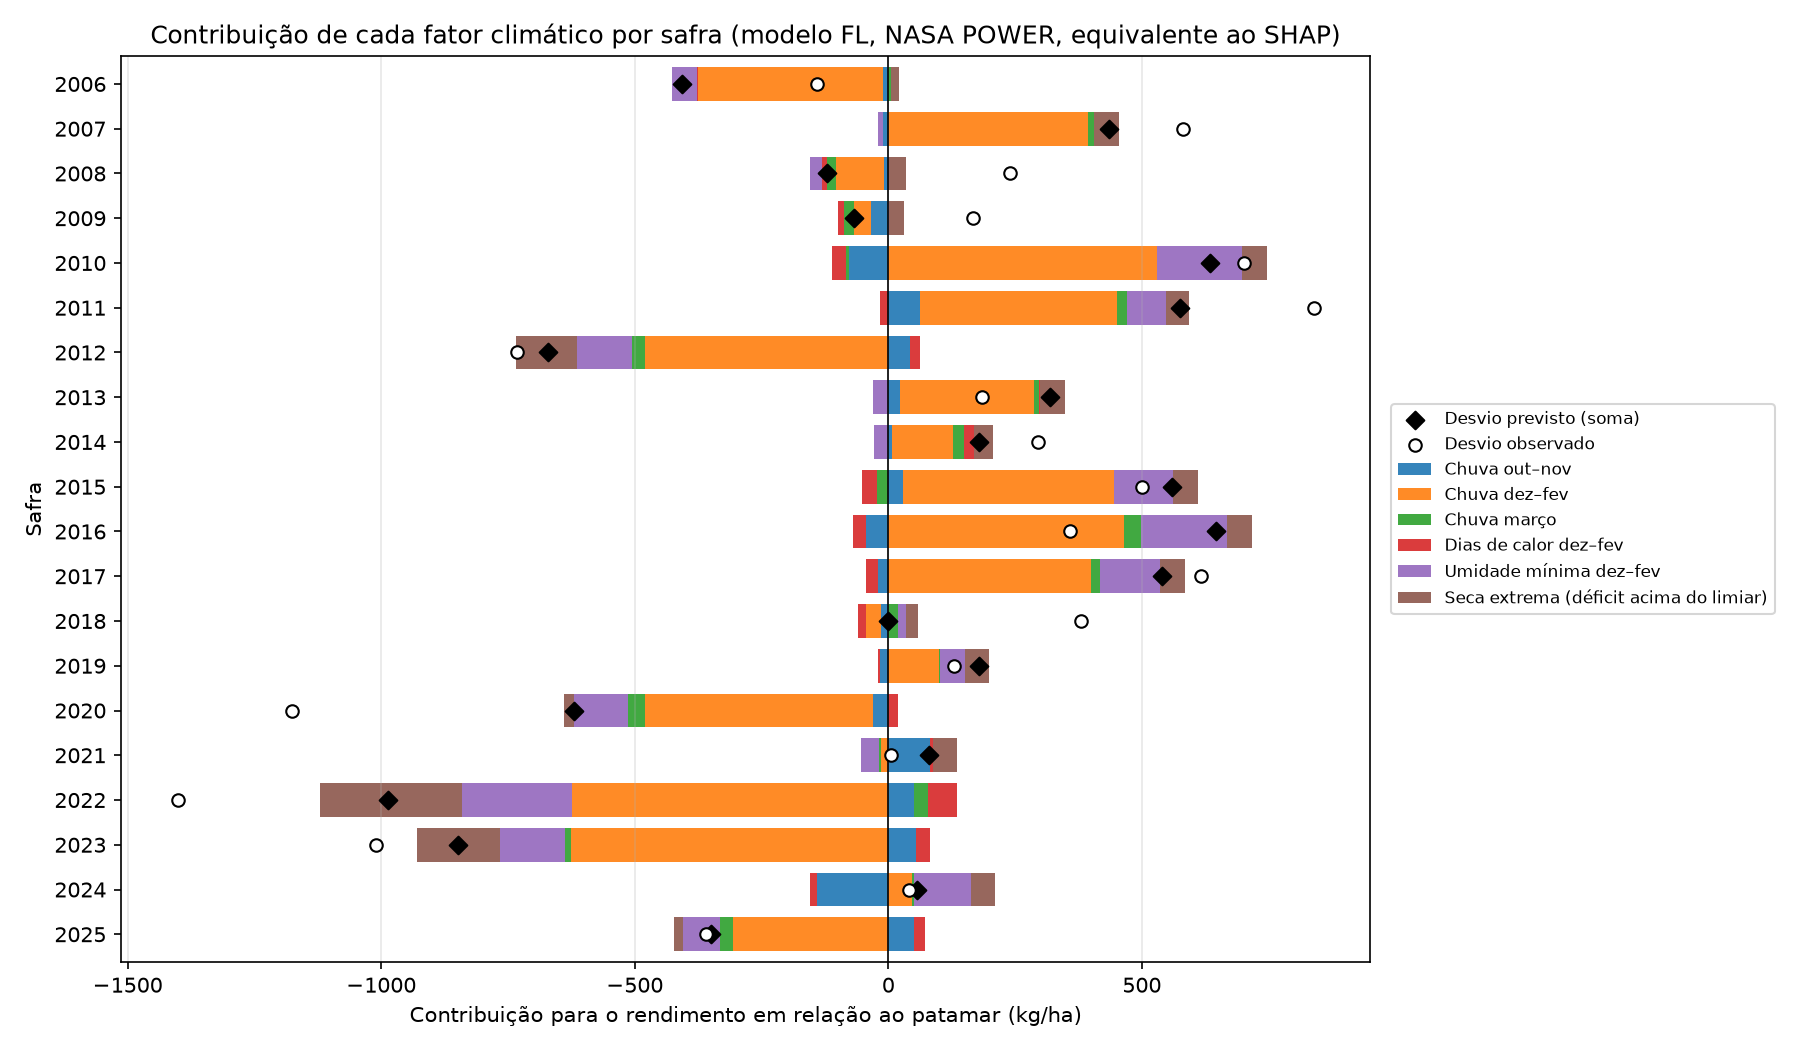
\includegraphics[width=0.95\textwidth]{figuras/fig4_contribuicao_fatores.png}
\fonte{Elaborado pelos autores (2026).}
\end{figure}

Nas safras previstas sem terem sido vistas pelo modelo, o FL captou 91\% da quebra de 2012, 81\% da de 2023, 38\% da de 2022 e 26\% da de 2020 (Figura \ref{fig:secas}). A quebra de 2020 ($\approx$1.000 kg/ha abaixo do patamar) é a menos captada: o verão foi apenas moderadamente seco, com primavera chuvosa. Parte das perdas de 2020 e 2022 não está nas variáveis disponíveis — possivelmente por chuva concentrada em poucos eventos ou por efeitos fora de dezembro--fevereiro —, o que caracteriza um limite de informação, e não de algoritmo.

\begin{figure}[htbp]
\centering
\caption{Desvio médio estadual em relação ao patamar, por safra, deixando uma safra de fora: observado e previsto pelos modelos F e FL}
\label{fig:secas}
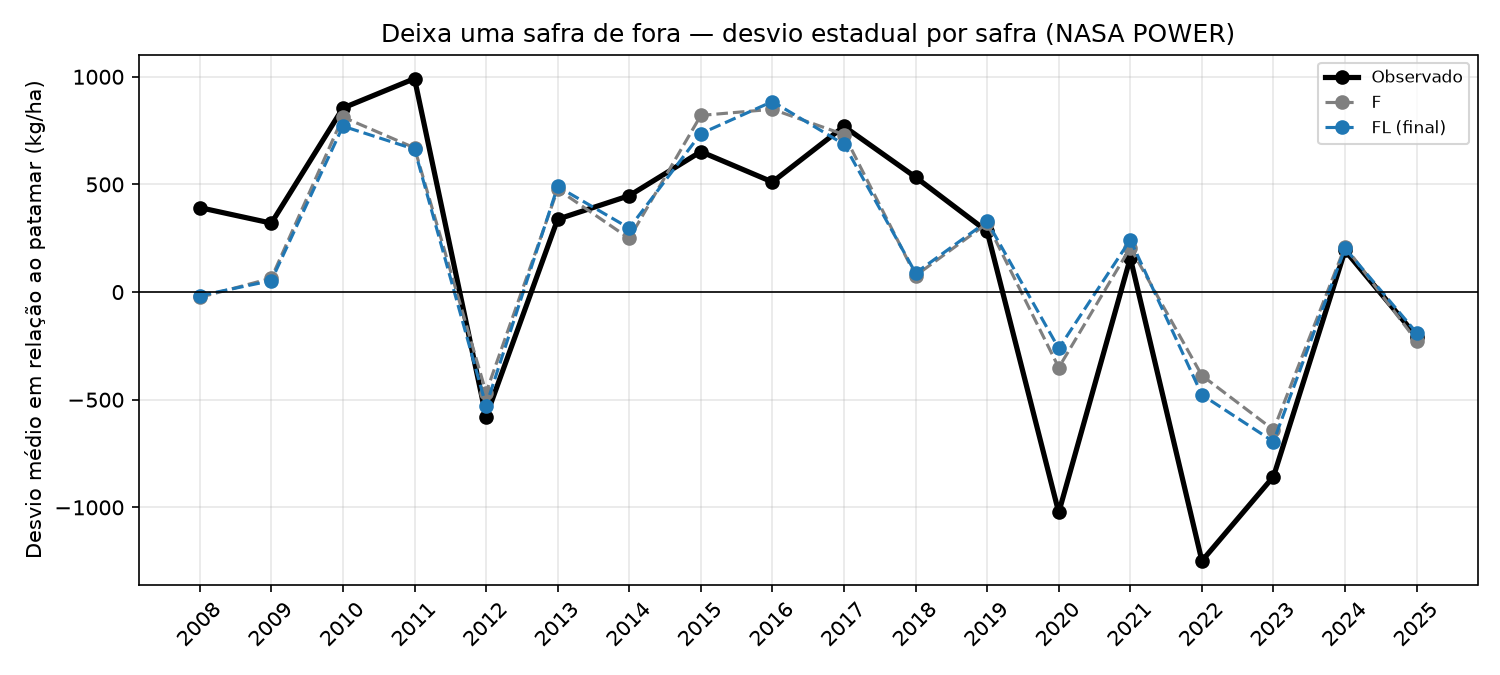
\includegraphics[width=0.95\textwidth]{figuras/fig5_secas_desvio_por_safra.png}
\fonte{Elaborado pelos autores (2026).}
\end{figure}

O erro relativo (MAE como percentual do rendimento médio, deixando uma safra de fora) foi menor no Nordeste (16,2\%) e no Noroeste (17,0\%), principal região produtora, e maior no Sudeste (28,0\%) e no Sudoeste (29,1\%), de produtividade média menor (Figura \ref{fig:regioes}). Entre os 424 municípios com pelo menos oito safras avaliadas, o erro relativo mediano foi de 17,9\% (metade entre 15\% e 22\%), e municípios mais produtivos tiveram erro relativo menor (correlação de $-$0,62).

\begin{figure}[htbp]
\centering
\caption{Erro relativo (MAE \% do rendimento médio) por mesorregião, nas duas validações (FL, NASA POWER)}
\label{fig:regioes}
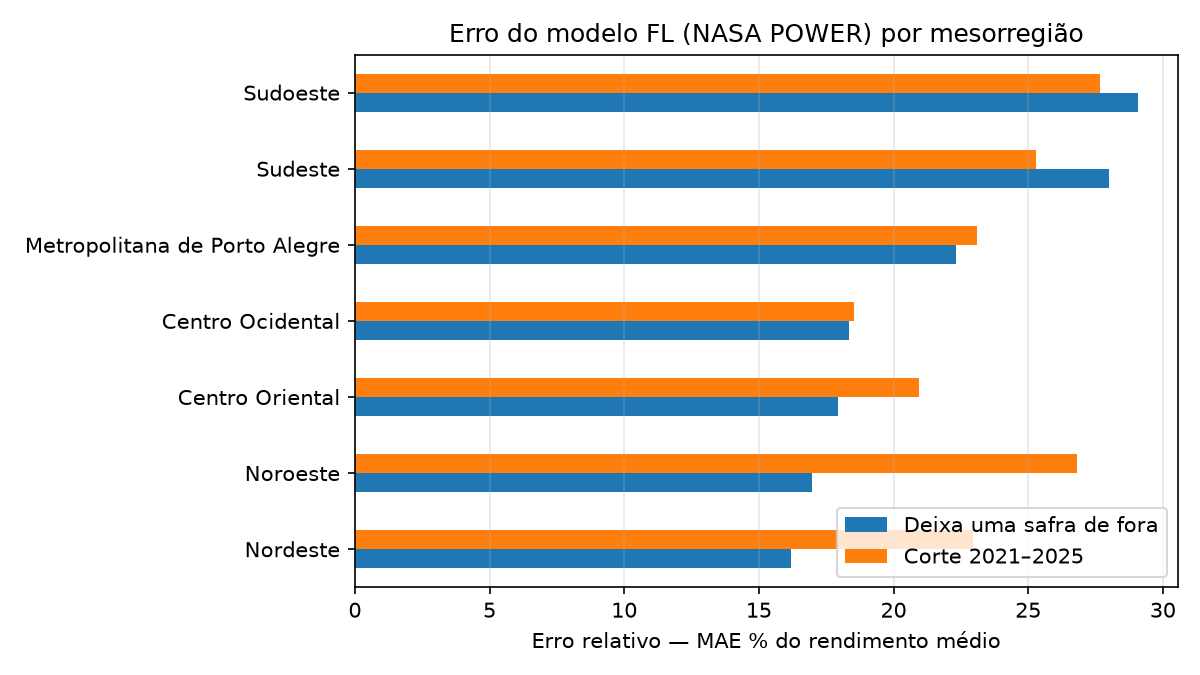
\includegraphics[width=0.75\textwidth]{figuras/fig6_erro_por_mesorregiao.png}
\fonte{Elaborado pelos autores (2026).}
\end{figure}

\subsection{Previsão da safra 2026}

O FL foi treinado com todas as safras de 2006 a 2025 e aplicado ao patamar 2020--2024 e ao clima de outubro de 2025 a março de 2026, nos 434 municípios que colheram soja em 2025. Pelo NASA POWER, a safra teve chuva bem abaixo da média em outubro--novembro (161 $\times$ 295 mm na média 2006--2025) e em dezembro--fevereiro (281 $\times$ 368 mm), com umidade mínima baixa (47\% $\times$ 52\%) e mais dias de calor (33 $\times$ 24); o déficit hídrico (245 mm) ficou abaixo do limiar de seca extrema, e o ONI médio da safra foi de $-$0,45 (fase neutra).

Com o patamar de 2.270 kg/ha (ponderado pela área), o FL prevê \textbf{2.097 kg/ha} para o estado, com intervalo de 80\% de 1.685 a 2.430 kg/ha (Tabela \ref{tab:prev2026}). A queda de 173 kg/ha em relação ao patamar vem principalmente da chuva de dezembro--fevereiro ($-$284 kg/ha) e da umidade mínima ($-$103 kg/ha), em parte compensadas pela chuva de outubro--novembro (+62 kg/ha) e pelo desvio médio do treino (+153 kg/ha). A queda se concentra no Sudoeste ($-$36\% sobre o patamar) e no Sudeste ($-$26\%), enquanto o Noroeste, com quase metade da área plantada, fica próximo do patamar ($-$1\%). A previsão de cada município está no arquivo \path{previsao_safra_2026_municipio.csv} do repositório.

\begin{table}[htbp]
\centering
\caption{Previsão do rendimento médio da soja no RS para a safra 2026 (kg/ha, ponderada pela área)}
\label{tab:prev2026}
\small
\begin{tabular}{|>{\raggedright\arraybackslash}p{7.00cm}|>{\centering\arraybackslash}p{2.60cm}|>{\centering\arraybackslash}p{3.60cm}|}
\hline
\textbf{Modelo} & \textbf{Previsão} & \textbf{Intervalo de 80\%} \\ \hline
\textbf{FL (final)} & \textbf{2.097} & \textbf{1.685 -- 2.430} \\ \hline
H2 & 2.094 & 1.649 -- 2.473 \\ \hline
F & 2.045 & 1.672 -- 2.387 \\ \hline
GB -- Gradient Boosting & 2.221 & 1.517 -- 2.682 \\ \hline
Média histórica & 2.276 & 1.833 -- 3.266 \\ \hline
Referência: patamar 2020--2024 & 2.270 & -- \\ \hline
Referência: LSPA/IBGE, set/2026 & 2.734 & -- \\ \hline
\end{tabular}
\fonte{Elaborado pelos autores (2026).}
\end{table}

O resultado oficial (PAM) da safra 2026 só será divulgado em setembro de 2027. A referência disponível é o Levantamento Sistemático da Produção Agrícola (LSPA) de setembro de 2026 \cite{ibgelspa}, que estima \textbf{2.734 kg/ha} e, em 2007--2025, ficou em média a 7 kg/ha da PAM (diferença máxima de 35 kg/ha). Em relação a ele, o FL subestimou a safra em cerca de 640 kg/ha ($-$23\%), fora do intervalo de 80\%, e todos os modelos ficaram abaixo do LSPA. É o primeiro teste totalmente fora da amostra do projeto, e indica que o clima de 2026 descrito pelo NASA POWER sugere um ano mais seco do que a safra mostrou — um problema da qualidade do clima de entrada, e não só do modelo. A perspectiva feita no plantio da safra 2026, com os cenários climáticos descritos a seguir, indicava mediana de 2.491 kg/ha e percentil 90 de 2.989 kg/ha, mais perto do LSPA.

\subsection{Perspectiva da safra 2027}

Em outubro de 2026, a soja de 2027 está sendo semeada. O patamar já é conhecido — média de 2021--2025, de 2.300 kg/ha, ainda baixo por incluir as secas de 2022, 2023 e 2025 —, mas o clima de dezembro a março, o que mais pesa no FL, ainda não aconteceu. O clima, portanto, não é previsto: o FL é aplicado ao patamar de 2027 com o clima observado em cada uma das 21 safras de 2006 a 2026 (cenários), separados pela fase do ENOS da safra de origem (ONI médio $\geq$ +0,5: El Niño; $\leq$ $-$0,5: La Niña). Como o ONI estava em +2,16 em julho--setembro de 2026, a safra 2027 deve ocorrer sob El Niño.

Com todos os cenários, a mediana é de 2.522 kg/ha; nos sete cenários de El Niño, sobe para \textbf{2.831 kg/ha}, acima do patamar e próxima das boas safras recentes (Tabela \ref{tab:prev2027} e Figura \ref{fig:prev}). O risco de quebra é menor, mas não nulo: o cenário de 2020, classificado como El Niño, resulta em 1.746 kg/ha, e o clima de La Niña de 2022 levaria a 1.195 kg/ha. Sob El Niño, todas as mesorregiões ficam acima do patamar, com maior ganho relativo no Sudoeste (+35\%) e no Centro Ocidental (+31\%). Como o FL subestimou 2026, essa perspectiva pode estar pessimista. A previsão propriamente dita será emitida em 31 de março de 2027, com o clima observado de outubro de 2026 a março de 2027.

\begin{table}[htbp]
\centering
\caption{Perspectiva do rendimento médio da soja no RS para a safra 2027 (kg/ha): FL aplicado ao patamar 2021--2025 com o clima de cada safra de 2006--2026}
\label{tab:prev2027}
\small
\begin{tabular}{|>{\raggedright\arraybackslash}p{2.43cm}|>{\centering\arraybackslash}p{1.54cm}|>{\centering\arraybackslash}p{1.54cm}|>{\centering\arraybackslash}p{1.54cm}|>{\centering\arraybackslash}p{1.54cm}|>{\centering\arraybackslash}p{1.54cm}|>{\centering\arraybackslash}p{1.54cm}|}
\hline
\textbf{Clima da safra} & \textbf{Cenários} & \textbf{Mínimo} & \textbf{Percentil 10} & \textbf{Mediana} & \textbf{Percentil 90} & \textbf{Máximo} \\ \hline
Todos & 21 & 1.195 & 1.623 & 2.522 & 3.019 & 3.077 \\ \hline
\textbf{El Niño} & \textbf{7} & \textbf{1.746} & \textbf{2.218} & \textbf{2.831} & \textbf{3.066} & \textbf{3.077} \\ \hline
Neutro & 5 & 1.897 & 1.989 & 2.594 & 2.884 & 2.977 \\ \hline
La Niña & 9 & 1.195 & 1.230 & 2.271 & 2.600 & 2.912 \\ \hline
\end{tabular}
\fonte{Elaborado pelos autores (2026).}
\end{table}

\begin{figure}[htbp]
\centering
\caption{Rendimento médio estadual observado, previsto na validação, previsão da safra 2026 e cenários da safra 2027 (FL)}
\label{fig:prev}
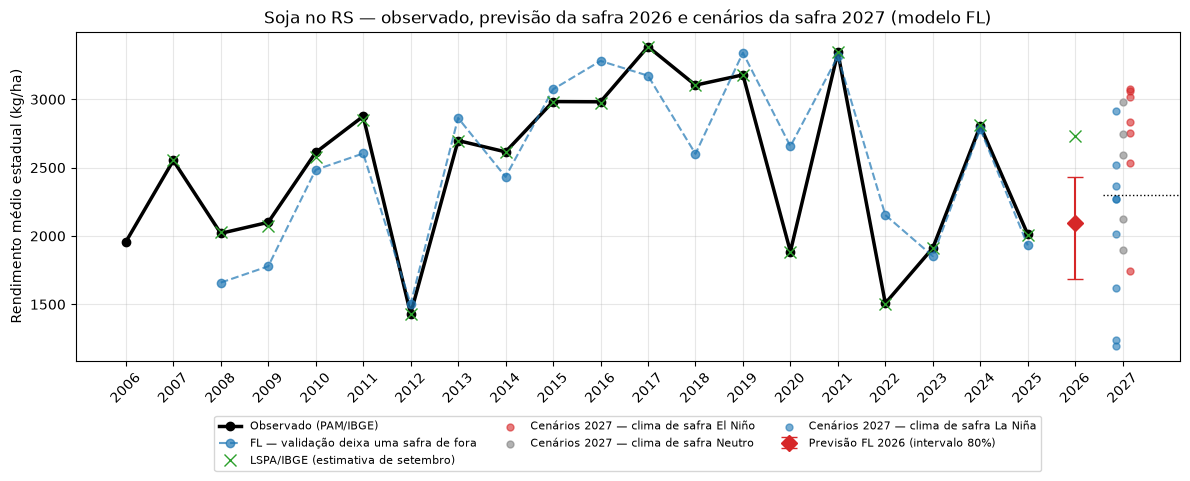
\includegraphics[width=0.95\textwidth]{figuras/fig7_previsao_2026_perspectiva_2027.png}
\fonte{Elaborado pelos autores a partir de IBGE, NASA POWER e NOAA (2026).}
\end{figure}

\subsection{Aplicação: recomendação de adubação}

Como aplicação complementar, o rendimento esperado foi combinado com as tabelas oficiais de recomendação para o RS e SC \cite{reuniao2014,sbcs2016} para gerar a dose de P\textsubscript{2}O\textsubscript{5} e K\textsubscript{2}O por classe de teor do nutriente no solo. Como a adubação é decidida no plantio, antes do clima do verão, o rendimento esperado usado é o patamar do município. Para a safra 2026, a dose no 1º cultivo em solo de teor ``Médio'' vai de 60 kg/ha de P\textsubscript{2}O\textsubscript{5} e 75 kg/ha de K\textsubscript{2}O no Sudoeste (rendimento esperado de 1.760 kg/ha) a 72 e 94 kg/ha no Nordeste (2.774 kg/ha). O resultado para 429 municípios está em \path{recomendacao_adubacao_safra2026.csv}; as doses são a recomendação normativa aplicada ao rendimento esperado, e o produtor identifica a sua classe pela análise de solo.

\subsection{Limitações e uso responsável}

O erro remanescente ($\approx$19\% por município, chegando a 29\% no Sudoeste) reflete limites de informação: a grade representa a média de uma área de $\approx$50 km, e não a lavoura; chuvas concentradas em poucos eventos não aparecem nos totais; e pragas, doenças, data de semeadura e manejo não estão nos dados. O próprio rendimento municipal da PAM é uma estimativa. O balanço hídrico usa uma CAD única de 75 mm e coeficiente de cultura igual a 1. A escolha do FL foi feita depois de testar seis variações nos mesmos dados; o ganho sobre o F é modesto ($\approx$3,5\% no RMSE médio), mas consistente nas duas validações e reconfirmado na Etapa 6. Os p-valores dos coeficientes tendem a ser otimistas, pois os municípios de uma mesma safra compartilham o mesmo ano climático.

O indicador não deve ser tomado como decisão automática de crédito, seguro ou plantio: decisões com impacto econômico devem envolver avaliação agronômica humana, e a previsão deve ser comunicada sempre com o seu intervalo. Código, versões das bases e parâmetros estão versionados no repositório para permitir auditoria e reprodução.

\section{Conclusão}\label{sec:conclusao}

Este trabalho investigou se é possível prever o rendimento da soja de cada município do Rio Grande do Sul em 31 de março, antes do fim da colheita e apenas com dados públicos já publicados nessa data. Para isso, integrou o rendimento municipal do IBGE, o clima do INMET e do NASA POWER, o ONI e um balanço hídrico do solo, e comparou regressão linear, Random Forest e Gradient Boosting com linhas de base históricas, em validações que respeitam a data de publicação dos dados.

A resposta é positiva, com ressalvas. O modelo final, FL — uma regressão linear que soma ao patamar do município um desvio explicado pela chuva, pela umidade e pela seca extrema —, erra $\approx$19\% por município e $\approx$244 kg/ha na média estadual, com erro 31\% menor que o da média histórica deixando uma safra de fora e 11\% menor no período de secas de 2021--2025. A hipótese inicial, de que os modelos \emph{ensemble} superariam a regressão linear, foi refutada: com cerca de 20 safras e secas mais extremas que as do histórico, os ganhos vieram da forma de representar o clima e o patamar — clima por subperíodo, patamar só com as safras publicadas, clima em grade e um termo de seca extrema —, e não da troca de algoritmo. A chuva e a umidade de dezembro a fevereiro são as variáveis mais associadas ao desvio do rendimento.

As contribuições são uma base municipal integrada e reprodutível, um protocolo de validação sem vazamento temporal e uma previsão real da safra 2026, que ficou 23\% abaixo da estimativa do IBGE e expôs a sensibilidade do modelo à qualidade do clima de entrada. Para 2027, sob o El Niño esperado, a perspectiva é de 2.831 kg/ha, acima do patamar de 2.300 kg/ha. As principais limitações são o erro ainda alto nas regiões de menor produtividade, a ausência de informações de manejo e de sanidade e a defasagem de publicação da PAM.

Como trabalhos futuros, recomenda-se validar o clima de entrada com as estações do INMET e com outra reanálise antes da previsão de 2027; testar índices de vegetação por satélite (NDVI) para captar perdas que o clima não explica, como as de 2020 e 2026; buscar uma estimativa antecipada do rendimento da safra anterior por município, que reduziria a defasagem do patamar; e reavaliar os modelos de árvores à medida que a série de safras crescer. Esses passos formam a base lógica para uma futura ferramenta de apoio à decisão, atualizada a cada safra.

% ----------------------------------------------------------
% ELEMENTOS PÓS-TEXTUAIS
% ----------------------------------------------------------
\postextual

\bibliography{referencias}

\end{document}
